\chapter{Introduction to Generative Adversarial Networks }
\label{chap:chapter1}

\begin{chapterabstract}
	In this chapter, we first propose an introduction to the problem of generative modeling and some solutions to tackle this problem. We then propose an overview of the Generative Adversarial Networks \citep{Goodfellow2014} framework, which is a recent method to train deep neural networks as generative models that is particularly adapted to the task of image generation. We will introduce some of its theoretical interpretations, as well as some of its variations and applications. We discuss the different limitations of this approach and expose three main goals among the different works: enhancing the visual quality of the generated samples; maintaining their diversity; and conditioning the model. We then discuss the recent advances that have been made to overcome some of these limitations and propose a taxonomy of these advances using the aforementioned directions. We discuss the evaluation of generative models and the difficulties of evaluating the intrinsic quality of a generated sample through an overview of the different classical metrics and discuss their limitations.
\end{chapterabstract}

\minitoc


\section{Generative modeling and adversarial learning}
Generative modeling with deep neural networks has been a challenging task due to the stochastic nature of sampling, which prevents the computation of gradient, thus preventing the classical training of a deep model with gradient descent. However recent approaches such as variational auto-encoders (\ac{VAE}s) \citep{Kingma2014b}, flow methods \citep{Dinh2017, Kingma2018} and adversarial models \citep{Goodfellow2014} managed to overcome this restriction. In this section, we first propose an introduction to generative modeling with a focus on latent variable models.

We will then focus on the Generative Adversarial Networks \citep{Goodfellow2014} framework, their training process  and some of their variants, especially their conditional and domain-transfer variants. We outline some limitations of this framework and propose a formulation of these limitations in the form of a trilemma between the intrinsic quality of the generated samples, their diversity and the quality of the conditioning of the model. With this tool, we propose a taxonomy of the recent \ac{GAN} approaches and identify trends in these approaches.


\subsection{Generative modeling with maximum likelihood estimation}

\begin{figure}
	\centering
	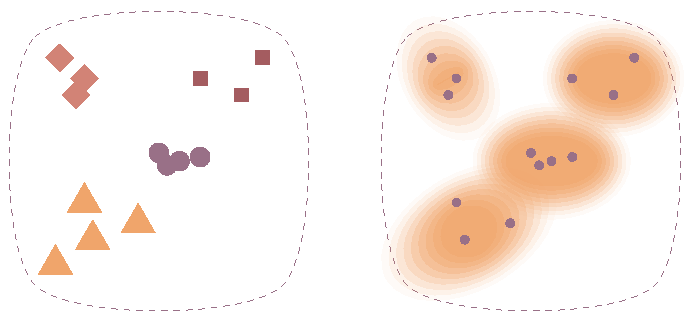
\includegraphics[width=\textwidth*3/4]{chapter1/disc_gen.pdf}
	\caption[Generative modeling]{Left: Discriminative modeling, the model aims to assign a class to each data point. Right: Generative modeling, the model aims to learn the underlying probability distribution of the data points.}
	\label{fig:disc_gen}
\end{figure}

Generative modeling is the task of learning the underlying distribution of a dataset in order to generate more samples from that distribution. In other words, it describes how data is generated in terms of a probabilistic model,  a distribution from which the whole dataset could have been sampled with a high likelihood.

 Indeed,  whereas a discriminative model tries to find decision boundaries by fitting a parametric model $\pt{Y|X}$  to a conditional probability distribution $\p{Y|X}$ of data $\vx\in\setX$ and labels $\vy \in \setY$ relatively to the data $\vx \sim \p{X}$, a generative model aims to fit $\pt{X}$ to $\p{X}$  the intrinsic distribution of the data and to provide a sampling mechanism on this distribution (\seefigure{fig:disc_gen}).

These two learning tasks, the discriminative (\citeq{eq:disc_mle}) modeling and the generative modeling (\ \citeq{eq:gen_mle}) can be formulated as a maximum log-likelihood estimation \\

\noindent\begin{minipage}{.5\linewidth}
	\begin{equation}
		\label{eq:disc_mle}
		\theta^* = \arg\max_\theta \esp{\vx,\vy\sim\p{y|x}} \log\pt{\vy|\vx}
	\end{equation}
\end{minipage}%
\begin{minipage}{.5\linewidth}
	\begin{equation}
			\label{eq:gen_mle}
		\theta^* = \arg\max_\theta \esp{\vx\sim\p{\vx}} \log\pt{\vx}
	\end{equation}
\end{minipage}\\

An simple example of generative model are Gaussian Mixture Models (\ac{GMM}) . They consist in a sum of $k$ Gaussian distributions $\mathcal{N}(\mu_i, \sigma_i^2), i \in 1..k$ which are all attributed a selection probability $\p{Z=i} = \pi_k$, with $\vz \in \setZ$, so that $\p{\vx|\vz=k} = \mathcal{N}(\mu_k, \sigma_k^2)$ . The model is then formulated as 

\begin{equation*}
	\pt{\vx} = \sum_{z}\p{z}\pt{\vx|z}\enspace,
\end{equation*}

with log-likelihood 

\begin{equation*}
	\log\sum_{\vx\sim\p{\vx}}\pt{x}  = \sum_{\vx\sim\p{\vx}}\log\sum_{k=1}^k \pi_k \mathcal{N}(\vx|\mu_k, \sigma_k^2)\enspace.
\end{equation*}

In the case of the \ac{GMM}s, the Expectation-Maximization (EM) algorithm \citep{Dempster1977} can be used to find the parameters $\theta^*$ which, at convergence, maximizes the log-likelihood of the model. Once the model is trained, sampling a new data is done by picking a component $k$ from the distribution $\p{\vz}$, then drawing a sample from the Gaussian distribution $\p{\vx|\vz=k} = \mathcal{N}(\mu_k^*, \sigma_k^{*2})$.

\subsection{Latent variable models}

\subsubsection{Latent variable models and marginalization}
For \ac{GMM}s, sampling a new point consists in, once the Gaussian component has been selected, sampling a point on a normal distribution.  This sampling can be done by using reparametrization: instead directly sampling $\vx \sim \mathcal{N}(\mu_k^*, \sigma_k^{*2})$, we can instead sample a latent variable $\vz \sim \mathcal{N}(0, 1)$ and compute $\vx = \G(\vz; \mu, \sigma) = \mu + \vz\sigma$.  Such a model, that consists in a deterministic function $\G: \setZ \rightarrow\setX$ with parameters $\theta$ applied to a random latent variable drawn from a fixed distribution $\p{\vz}$ is a latent variable model.

\begin{figure}
	\centering
	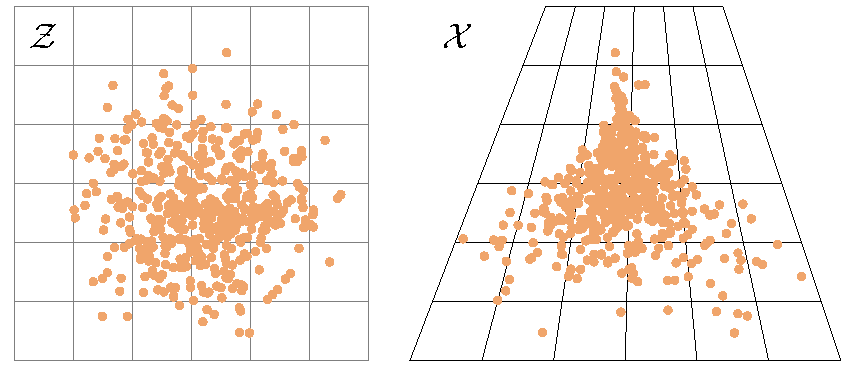
\includegraphics[width=\textwidth*3/4]{chapter1/latent_model.pdf}
	\caption[Latent variable model]{\CR{A refaire :/ n}A mapping between a latent space $\setZ$ and the space of a dataset $\setX$.}
\end{figure}

Since more complex distributions does not necessarily provide a natural sampling mechanism, using a latent variable model allows to outsource the stochastic part of the sampling  process from the learning process and only learn the function $\G(\vz; \theta)$. More formally, instead of directly modeling $\p{\vx}$, a latent variable model learns a deterministic mapping $\pg{\vx|\vz}$. From this mapping, the generative model can be obtain through marginalization 

\begin{equation}
	\pg{\vx} = \int_\setZ \p{\vz} \pg{\vx|\vz} d\vz = \int_\setZ \p{\vz} \p{\vx | G(\vz;\theta)} d\vz \enspace .
\end{equation}

This marginalization allows for the use of an arbitrary flexible $\G$. However, if $\G$ is non-linear, the actual evaluation of $\pg{\vx}$ is very likely to be intractable due to the integral over $\setZ$, which prevents the training of such a model as is.

While the marginal distribution $\pg{\vx}$ cannot be explicitly computed for any function $\G$, several solutions exist to overcome this problem and train deep generative models with latent variables anyways.  

\subsubsection{Variational auto-encoders}
\label{sub:deep_gen_modeling}

Variational Auto-Encoders (\ac{VAE}) \citep{Kingma2014b}  are deep latent variable models which tackle the marginalization problem by approximating the integral using a variational approach. To this end, they both learn the distribution of the latent model $\pg{\vx | \vz}$ as well as the distribution $\qf{\vz|\vx}$. This is done with  with two different neural networks, a decoder network  $\G:\setZ\rightarrow\setX$   and an encoder network $\F: \setX\rightarrow\setZ$ and allows to compute the distribution $\p{\vx}$ as

\begin{equation*}
	\log\pg{x} -  \DKL{\qf{\vz|\vx}}{\p{\vz|\vx}} = \esp{\vz\sim\qf{\vz|\vx}}\big[\log\pg{\vx|\vz}\big] - \DKL{\qf{\vz\vx}}{\p{\vz}}  \enspace .
\end{equation*}

The KL terms evaluates the distance between the distribution $\qf{\vz|\vx}$ learned by the encoder and real distribution $\p{\vz|\vx}$, and since $\p{\vz}$ is chosen Gaussian, this KL terms can be explicitly computed. The first term, is equivalent to the reconstruction error of an auto-encoder. Hence the model is trained by minimizing 

\begin{equation*}
	L_{VAE}(\F, \G) = \esp{\vz \sim \qf{\vz|\vx}}\big[ ||x - \G(\vz)||^2_2 \big] - \DKL{\qf{\vz|\vx}}{\p{\vz}}
\end{equation*}

However, since sampling $\vz \sim\qf{\vz|\vx}$ is not differentiable, the \ac{VAE} uses the so-called \textit{reparametrization trick}, that is to have $\F(\vx)$ output the mean and the variance $(\mu_\vx, \sigma^2_\vx)$ of a normal distribution for a sample $\vx$, so that a $\epsilon \sim  \mathcal{N}(0,1)$  is sampled outside of the model and given as a parameter, thus allowing to compute $\vz = \mu_\vx+\sigma_\vx\epsilon$, which is differentiable by considering $\epsilon$ a parameter.

\begin{figure}
	\centering
	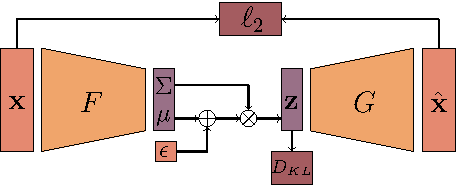
\includegraphics[width=\textwidth*3/4]{chapter1/vae.pdf}	%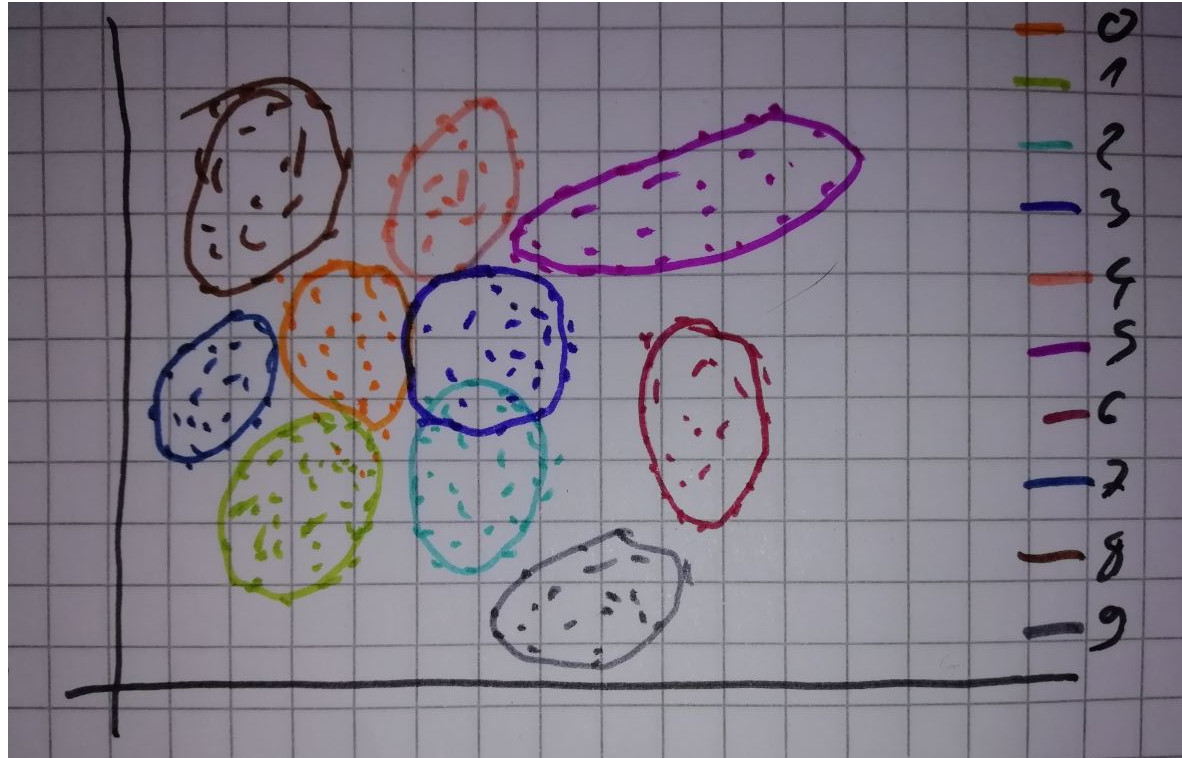
\includegraphics[height=\textheight/5,width=\textwidth*2/5]{chapter1/vae_latent.jpg}
	\caption[Variational auto-encoder]{ Variational auto-encoder framework}
\end{figure}

Finally, generating a sample $\vx$ with the trained model can be done by sampling a random vector $\epsilon \sim  \mathcal{N}(0,1)$ and computing $\vx = \G(\vz)$.

\subsubsection{Normalizing flows}

Normalizing flow based techniques is a family of latent variable models that aim to tackle the marginalization problem by using the \textit{change of variable formula}

\begin{equation*}
	\pg{\vx} = \p{\vz} \Big|\det\Big(\frac{\partial\G(\vz)}{\partial{\vz^T}}\Big)\Big|^{-1}  = \p{\G^{-1}(\vx)} \Big|\det\Big(\frac{\partial\G^{-1}(\vx)}{\partial{\vx^T}}\Big)\Big|  \enspace ,
\end{equation*}
with $\vz \sim \p{\vz}$ a latent variable. This formulation has notable advantages such as explicitly allowing the computation of the exact inference. However, the model has to enforce some tough constraints: the input and output dimensions must be the same; $\G$ must be invertible; and computing the determinant of the Jacobian needs to be efficient and differentiable.

These constraints can be enforced through strong restrictions on the architecture of the model. By limiting the transformations to a set of invertible transformations with a tractable Jacobian determinant, the model remains invertible and the determinant of its Jacobian can be computed efficiently. 

Real-valued non-volume preserving (RealNVP) normalizing flows \citep{Dinh2017} uses affine coupling transformations, which transforms a variable by adding and scaling it by a non-linear transformation of itself, usually computed with deep neural networks. These transformations can be inverted by substracting and downscaling by the same transformed variables and their Jacobian is triangular, therefore computing its determinant can be done efficiently by computing the product of its diagonal terms.  \textit{Glow} \citep{Kingma2018} extended this set of transformations to $1\times1$ invertible convolutions as well as a variant of batch normalization that allows for more expressiveness in the model.

%$\vx$ into $\vy$ by partitioning it into $(\vx_1, \vx_2)$ and computing $\vy_1 = \vx_1; \vy_2 = \exp(s_\theta(\vx_1)) \odot \vx_2 + m_\theta(\vx_1)$, where $s_\theta$ and $m_\theta$ are arbitrary scaling and translation parametric functions. These transformations can be inverted as $\vx_1 = \vy_1; \vx_2 = \exp(-s_\theta(\vy_1)) \odot (\vx_2 - m_\theta(\vx_1))$ 




\subsection{Generative Adversarial Networks}

In the same fashion as the generative models mentioned in \citesub{sub:deep_gen_modeling}, Generative Adversarial Networks (\ac{GANs}) \citep{Goodfellow2014} aims to learn a parameterized mapping $\pg{\vx|\vz}$ between a simple distribution $\p{\vz}$ (usually normal or uniform) to the real data distribution $\p{\vx}$. However, instead of relying on the likelihood and trying to estimate the distribution through marginalization, it aims to minimize an estimation of a divergence between $\p{\vx}$ and the mapped distribution $\pg{\vx}$.  Therefore, \ac{GANs} are often qualified as \textit{likelihood-free} generative models.

\begin{figure}
	\centering
	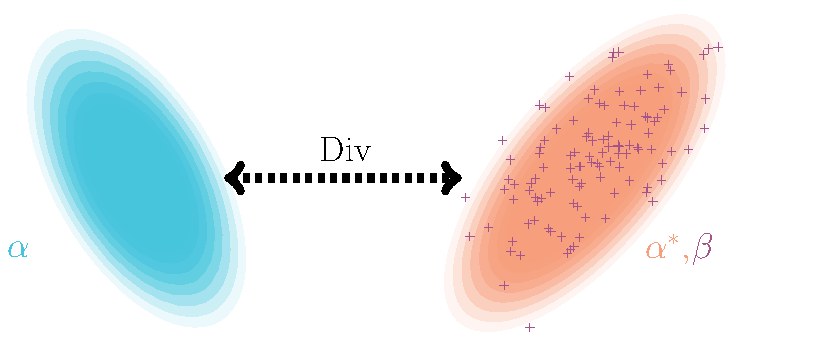
\includegraphics[width=\textwidth*3/4]{chapter1/div.pdf}\hspace{-2cm}
	\caption[Illustration of a divergence]{A divergence $\Div{\alpha_\theta}{\beta}$ can capture the distance between a parametric model $\alpha_\theta$ and the observations $\beta$. Density fitting can then be formulated as  finding $\theta^* = \arg\min_\theta \Div{\alpha_\theta}{\beta}$, such that $\alpha_{\theta^*}$ is the best fit model.}
	\label{fig:divergence}
\end{figure}


Since a divergence $\Div{\p{\vx}}{\q{\vx}}$ between two distributions $\p{\vx}$ and $\q{\vx}$ is analogous to a distance between these distributions (\seefigure{fig:divergence}), minimizing such a divergence allows for a parametric distribution $\pt{\vx}$ to fit a target distribution $\p{\vx}$. When this divergence is both tractable (or estimable) and differentiable w.r.t the parameters $\theta$, it can be directly optimized, allowing for the training of a generative model.

However in practice, such divergences usually intractable in the case of generic distributions. \ac{GAN}s aim to estimate this divergence by relying on a second learned function that will act as a surrogate to the divergence, the discriminator model $\D$. This discriminator is a binary classifier that aims to predict the probability that a sample $\vx$ was sampled on the real distribution $\p{\vx}$ or was  generated from $z\sim\p{\vz}$ and is trained with binary cross-entropy

\begin{equation*}
	L_\D(\D, \G) =  \esp{x\sim \p{\vx}} [\log \D(x)] +  \esp{\vx\sim\pg{\vx}} [1 - \log \D(\vx)] \enspace .
\end{equation*}

The intuition behind this model is that once the discriminator is trained, maximizing its error on generated samples $\vx\sim\pg{\vx}$ w.r.t the parameters of $\G$ should push $\pg{x}$ towards $\p{x}$.

\begin{figure}
	\centering
	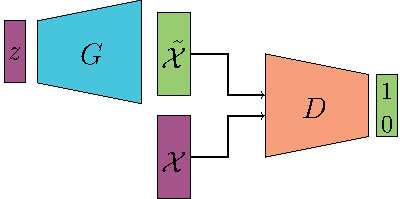
\includegraphics[width=\textwidth*2/3]{chapter1/gan.pdf}
	\caption{Generative Adversarial Networks framework}
\end{figure}

The minimum of $f(x) = a\log(x) + b\log(1-x)$ is $\frac{a}{a+b}$, so the discriminator that maximizes $L_\D(\D, \G)$ for a fixed $\G$ is given by

\begin{equation*}
\label{eq:optimal_D}
\D^*_\G(x) = \frac{\p{\vx}}{\p{\vx} + \pg{\vx}} \enspace.
\end{equation*}

By plugging this optimal into the discriminator cost, we get
\begin{equation*}
		\min_\D L_\D(\D,\G) =  \esp{x\sim \p{\vx}} \Big[\log \frac{\p{\vx}}{\p{\vx} + \pg{\vx}}\Big] +   \esp{{x}\sim \pg{\vx}} \Big[1 - \log  \frac{\pg{\vx}}{\p{\vx} + \pg{\vx}}\Big] \nonumber \enspace.
\end{equation*}

As said previously, the objective of the generator model $\G$ will be to maximize the error of the discriminator $\D$. Thus, we can formulate a criterion $L_\G(\G)$ as $L_\G(\G) = \min_\D L_\D(\D,\G)$. Up to additive and multiplicative constants, the criterion  $L_\G(\G)$ can be reformulated as

\begin{equation*}
		L_\G(\G) = \DKL{\p{\vx}}{\frac{\p{\vx}+\pg{\vx}}{2}} + \DKL{\pg{\vx}}{\frac{\p{\vx}+\pg{\vx}}{2} } = 2\cdot\JSD{\p{\vx}}{\pg{\vx}} \enspace.
\end{equation*}

When the discriminator is trained to convergence, minimizing the criterion $L_\G( \G) = \lgan(\D^*, \G)$ is equivalent to minimizing the Jensen-Shannon (\ac{JS}) divergence between $\p{\vx}$ and $\pg{\vx}$.  This training process is summed up as a mini-max game in \citeq{eq:GAN_problem} 

\begin{equation}
\label{eq:GAN_problem}
\arg\min_\G\max_\D\lgan = \arg\min_G\max_\D \esp{x\sim \p{\vx}} [\log \D(x)] +  \esp{z\sim\p{\vz}} [1 - \log \D(\G(z))] \enspace.
\end{equation}

As shown above, this mini-max game has, assuming infinite capacity for both $G$ and $D$, a global optimum for $\p{\vx} = \pg{\vx}$. The \ac{GAN} training algorithm then consists in alternatively updating the discriminator and the generator via gradient ascent/descent. A summary of this process is presented in \citealg{alg:GAN_train}. 

\begin{algorithm}[!ht]
	\caption{The \ac{GAN} training algorithm}
	\label{alg:GAN_train}
	\begin{algorithmic}[H]
		\REQUIRE{$\trainsetX$ the real dataset, $G$ the generator model, and $D$ the discriminator model}
		\REPEAT
		\STATE sample a mini-batch $\lbrace x_i \rbrace_{i=1}^m$ from $\trainsetX$\;
		\STATE sample a mini-batch $\lbrace z_i \rbrace_{i=1}^m$ from $\p{\vz}$\;
		\STATE update $D$ by stochastic gradient ascent of
		\STATE \ \ \ \ $ \sum_{i=1}^{m}\log(D(x_i)) + \log(1-D(G(z_i)))$
		\STATE sample a a mini-batch $\lbrace z_j \rbrace_{j=1}^n$ from distribution $\p{\vz}$\;; 
		\STATE update $G$ by stochastic gradient descent of
		\STATE \ \ \ \ $ \sum_{j=1}^n \log(1-D(G(z_j)))$\;
		\UNTIL a stopping condition is met
		
	\end{algorithmic}
\end{algorithm}

\subsection{Limitations}
\label{sub:limitations}

GANs have shown strong advantages over the classical generative modeling methods, such as generating sharper samples than \ac{VAE}s and normalizing flows \citep{Danihelka2017}. They however bear limitations, namely: the instability of the training process; the loss of diversity in the generated samples (\textit{mode-collapse}); and finally the problem of black-box conditioning. 

\subsubsection{Instability}

As we have seen in the previous section, training \ac{GAN}s consist in solving a minimax problem. While the alternate gradient descent algorithm is a straightforward method for solving such a problem, the alternating updates can cause significant instabilities during the training process. This can result in oscillating values of the loss function which prevents convergence \citep{Mescheder2018}, which makes it difficult to determine a when to stop training. In the end, this behavior can be harmful in terms of performance.

\CR{Figure loss GAN}

The instability of the \ac{GAN} training process has first been conjectured to be caused by the bad quality of the gradients obtained when $\G$ generates bad samples, which makes $\D$ strongly reject these samples and therefore saturating the loss. The first solution proposed \citep{Goodfellow2014} was to slightly change the generator's loss function from $\log(1-\D(\G(z)))$ to $-\log(\D(\G(z)))$, which helped considerably in avoiding failures of the training process and was then widely used \citep{Radford2015} \CR{Plus de citations}.

 While this loss term converges to the same minimum as the original loss term, minimizing it no longer correspond to minimizing a \ac{JS} divergence but the non-symmetric reverse \ac{KL} divergence (minus a \ac{JS} term) \citep{Arjovsky2017a}. More formally, 

\begin{equation*}
	\esp{\vz\sim\p{\vz}}\Big[\nabla_\G\log\D^*(\G(\vz))\Big] = \nabla_\G\Big[\DKL{\pg{\vx}}{\p{x}} - 2\JSD{\pg{\vx}}{\p{x}}\Big] \enspace .
\end{equation*}

\begin{figure}
	\centering
	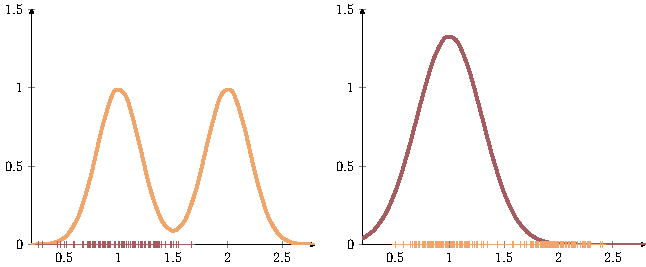
\includegraphics[width=\textwidth]{chapter1/kl_rkl.pdf}
	\caption[\ac{KL} and reverse \ac{KL} divergence]{Reverse \ac{KL} (left) and \ac{KL} (right) divergence between the true blue distribution and the mode-collapsed orange distribution . The distance is lower in the case of the reverse \ac{KL}, even if a missing mode is clearly visible.}
	\label{fig:kl_rkl}
\end{figure}

However, albeit an empirical reduction of the instability, this loss substitution has been proved to not solve the instability problem \citep{Arjovsky2017a}. This is mainly due to an unstable behavior of these divergences when the real distribution and the learned one does not share the same support.

 A lot of similar tricks can be applied to the training process in order to avoid this pitfall \citep{Salimans2016, Sonderby2017, Heusel2017},  and while more recent approaches seemed to help alleviate this issue (which will be more detailed in the next section), instability can still be observed in the most recent approaches \citep{Brock2018}. Even though several theory-backed techniques aimed to solve this issue \citep{Arjovsky2017, Nowozin2016, Li2017a}, there are still, at the time of writing this thesis, neither clear consensus on the theoretical causes of this instability nor completely efficient solutions.


\subsubsection{Mode collapse}
\label{subs:mode_collapse}

Although the aforementioned change of loss can help solving the instability issues, using the reverse \ac{KL} divergence is conjectured to be one of the causes of another issue: the \textit{mode collapse} problem: different $\vz_1, \vz_2$ are mapped to samples $\G(\vz_1)$ and $\G(\vz_2)$ that are very close;  and  \textit{mode dropping}: only a localized subset of the distribution can actually be mapped to, leading to missing modes in the generated samples.

Indeed, the reverse \ac{KL} divergence does not penalize "missing" parts of the learned distribution $\pg{\vx}$, which are some points in the support of $\p{\vx}$ that have zero (or near-zero) probability on $\pg{\vx}$ (\seefigure{fig:kl_rkl}).

Another conjectured cause is raised by the alternate gradient descent, in that it does not clearly prioritize the minimax formulation $\G^* = \min_\G\max_\D \lgan$ over the maximin formulation $\G^* = \max_\D\min_\G \lgan$, which does not behave in the fashion as it pushes the generator towards mapping every $\vz$ to the single most probable $\vx$, evaluated  by the generator \citep{Goodfellow2016}.

In the same fashion as the instability problem, there is at the time of writing this thesis no fundamental explanation to this issue. However, it still raise a first trade-off: since using the original \ac{GAN} creates instability which lead to a drop of visual quality, and using the non-saturating variant creates a lack of diversity. This extends to more recent approaches in which higher visual quality induces a loss of diversity \citep{Brock2018}.

In the most extreme cases, this loss of diversity can result in a complete collapsing of the sampling mechanism, making it completely impossible to draw diverse samples. However this is not as much of an issue for conditional tasks that consists in mapping an input to one of many acceptable outputs, with one example of such a task being domain-transfer (see \citesec{subsec:domain_transfer}). 

\subsection{A note on the  evaluation of  GANs}
\label{subs:evaluation_methods}

Unlike discriminative models, evaluating and comparing \ac{GAN} approaches is a non-trivial task. Two approaches can be envisioned: evaluating the \textit{intrinsic} quality of generated samples with ad-hoc criterions or directly evaluating the likelihood of the generated samples. However, unlike \ac{VAE}s and flow-based models, \ac{GAN}s offer no explicit way to evaluate or approximate the likelihood of the generated samples. Thus, a significant part of the \ac{GAN} literature resorted to a subjective visual evaluation of the generated samples. 

In order to provide a more precise evaluation of the visual quality of generated samples, two ad-hoc methods Inception Score (\ac{IS}) \citep{Salimans2016} and Fréchet Inception Distance (\ac{FID}) \citep{Heusel2017} were proposed, which both make use of a pre-trained Inception v3 model \citep{Szegedy2016}, a deep classifier trained on the ImageNet dataset \citep{Deng2009}.

\textbf{Inception Score (\ac{IS})}) \citep{Salimans2016} is based on the evaluation of the entropy of the labels $\vy$ predicted by the Inception classifier of generated data. High-fidelity samples should be easier to classify and therefore have a conditional label distribution $\pg{\vy|\vx}$ with low entropy. In addition to the high quality, the samples should be diverse, therefore the marginal distribution $\pg{\vy} = \int_{\setZ}\pg{\vy|\vx=\G(\vz)}d\vz$ should have a high entropy. By combining these two requirements, the \ac{IS} is formulated as 

\begin{equation*}
	\text{IS}(\vy) = \exp\Big[\esp{\vx\sim\pg{\vx}} \DKL{\pg{\vy | \vx}}{\pg{\vy}}\Big] \enspace .
\end{equation*}

Although it has been widely used, \ac{IS} has shown major issues \citep{Barratt2018} that raise from the use of the conditional label distribution. Most notably, examples that are correctly classified are not necessarily of the highest quality and the pre-determined label classes can skew the estimation of the marginal distribution $p_\G(\vy)$.

The \textbf{Fréchet Inception Distance (\ac{FID})} \citep{Heusel2017}  differs from \ac{IS} since it evaluates a distance between the distributions of visual features computed on real and generated data, instead of relying on the labels. These features are extracted at the penultimate layer of the Inception classifier. The distributions of these features are assumed Gaussian, so that the Fréchet distance (or Wasserstein-2 distance) can be computed as
\begin{equation*}
	FID = ||\mu – \mu_G||^2 + Tr(\Sigma + \Sigma_G – 2\sqrt{\Sigma\times\Sigma_G}) \enspace ,
\end{equation*}

where $\mathcal{N}(\mu, \Sigma)$ and $\mathcal{N}(\mu_G, \Sigma_G)$ are the distributions of the extracted features of the real and generated data, respectively. \ac{FID} is considered more robust than 
\ac{IS} and has been either completing or replacing the use of \ac{IS} in recent works.

However, while these two metrics are considered to be the standard method for evaluating \ac{GAN}s, their reliance on the pre-trained Inception model can prove to be an issue. Indeed, they behave well when used to compare models learned on natural images datasets such as ImageNet, but they cannot directly be applied to other datasets. A solution to consider can be the training of another classifier network on a more adapted dataset, but this solution cannot be applied when no labeled data is available.

For completeness, we can also refer to notable (albeit less used) among numerous others metrics for evaluating visual quality  \citep{Borji2018}: the Parzen window (or kernel density) estimation \citep{Parzen1962} aim to estimate the likelihood of the generated samples; the Sliced Wasserstein Distance \citep{Julien2011} is an efficient approximation of the Earth-Mover (or Wasserstein) distance; the  Kernel Inception Distance \citep{Binkowski2018} is a recent metric that evaluates the maximum mean discrepancy between Inception features with a polynomial kernel.

Finally it is to note that for conditioned models, evaluating the aforementioned metrics does not inform about the quality of the conditioning. However, since the conditioning usually requires either labels or prior information, these can often be evaluated by, for example, predicting the labels of generated samples with a pre-trained classifier and computing the error between the predicted label and the original one.


\section{The GAN Zoo}

Recently, Generative Adversarial Networks have made considerable progress towards generating realistic high definition images \citep{Brock2018, Karras2020, Wang2018b}. These notable successes leverage on an overwhelming amount of incremental enhancements and variations of the original GAN \citep{Hindupur2017} that has been made in the recent years. In this section, a summary of these GAN variants is proposed by examining different three objectives: conditioning the generation, enhancing the visual quality of the generated samples, ensuring some diversity among the generated samples. We propose a classification of these approaches into three categories: alternative and additional losses for conditioning;  changes to the original objective functions; and improvements to the  architecture, regularization, normalization and training process. A summary of this overview is presented in \citefig{fig:trilemma}.



\subsubsection{Domain-transfer}

\CR{Moved to chapter 3}

\ac{CGAN}s \citep{Mirza2014} (see section \ref{sec:chap1cgan}) already learn to model the conditional distribution $\p{\vx|\vy}$, and adding a way to enforce the consistency of the semantic information enables domain-transfer.

Pix2Pix \citep{Isola2016} implemented this approach  explicitly by using paired samples $(\vx, \vy) \sim \p{\vx|\vy}$ forcing the generator to minimize the $\Lone$ reconstruction term between $x$ and $\G(y,z)$

\begin{equation*}
	\arg\min_G\max_\D L_{p2p} =  \arg\min_G\max_\D \lcgan(\D, \G) +\lambda\esp{x\sim\p{\vx}\\y\sim\p{\vy}\\z\sim\p{\vz}} ||x - G(y, z)||_1 \enspace .
\end{equation*}

However, this kind of approaches rely on paired data which can be very hard to obtain, especially in the case of natural images. When trying for example to transfer images of zebras to images of horses, you need a dataset of very similar zebras and horses in the exact same position for the $\Lone$ term to work.

\subsubsection{Task-specific losses}

\CR{TODO} %TODO Subsection class specific losses

\subsection{Objective variants}

As mentioned in \citesub{sub:limitations}, the original GAN losses as well as the non-saturating losses show strong limitations, the former causes instability and the latter causes a loss in diversity. As a possible solution to these issues, several new loss terms were envisioned

\subsubsection{Changing the divergence}
\label{sec:divergences}

As an alternative to the original loss and in order to replace the Jensen-Shannon and the reverse Kullback-Leibler divergences as objectives, the Least-Squares GAN (\ac{LSGAN}) \citep{Mao2017} were proposed. In this approach, the loss function are replaced with a least-square formulation of the discriminator error, as 

\begin{equation*}
	\loss{LSGAN}(\D, \G) = \esp{\vx\sim\p{\vx}} \Big[ (1-\D(\vx))^2\Big] + \esp{\vz\sim\p{\vz}} \Big[ (\D(\G(\vz)))^2\Big] \enspace .
\end{equation*}

While this loss function follow the same idea as the original GAN method, \ac{LSGAN} actually optimizes the Pearson's $\chi^2$ divergence. Empirically, \ac{LSGAN}s show more stability as well as a higher visual quality of the generated samples than the original GAN approach, which have been conjectured to be caused by a better quality of the gradients.

Although showing notable differences in their behavior when optimized, both the Jensen-Shannon, reverse Kullback-Leibler and Pearson $\chi^2$ divergences are part of the $f$-divergence family \citep{Liese2006} defined as 

\begin{equation*}
	D_f(p || q)  =\esp{\vx\sim\q{\vx}}f\Big(\frac{p(x)}{q(x)}\Big)  \enspace ,
\end{equation*}

where $f: \mathbb{R}^+\rightarrow \mathbb{R}$  is a convex, lower-semicontinuous function satisfying $f(1) = 0$. By carefully choosing $f$, we can recover the \ac{KL} ($f(u) =  u\log u$), reverse \ac{KL} ($f(u) =  -\log u$), \ac{JS} ($f(u) =  -(u+1)\log (\frac{u+1}{2} + u\log u)$) and Pearson's $\chi^2$ ($f(u) = (u-1)^1$) divergences. \citet{Nowozin2016} proposed a generalized approach for these divergences as well as several new GAN formulation based on divergences such as the Squared Hellinger distance or the Total Variation, which has been shown \citep{Arjovsky2017} to be the divergence used in the Energy-Based GAN \citep{Zhao2017} approach.  

While the $f$-divergences have been the seminal approach to GANs, they can exhibit strong issues. \citet{Arjovsky2017} have shown that these divergences can have degenerate behavior, most notably in the case where the two distributions have no shared support, which is reflected by points where the divergence is non-continuous and non-differentiable.

As a solution to this issue and orthogonal to the $f$-divergences, \citet{Arjovsky2017} proposed the Wasserstein GAN (\ac{WGAN}), replacing the Jensen-Shannon divergence by the Wasserstein -1 (or Earth-Mover) distance, which stems from transportation theory \citep{Peyre2020}.  The Wasserstein distance, albeit having many different formulations, can be expressed through the Kantorovich-Rubinstein duality \citep{Kantorovich1982} as

\begin{equation*}
		W(p||q) = \sup_{f \in \mathcal{F}} \Big[ \esp{\vx\sim\p{\vx}} f(\vx) - \esp{\vx\sim\q{\vx}} f(\vx) \Big] \enspace ,
\end{equation*}

where $\mathbb{F} = \{f:||f||_L\leq1\}$ is the set of all 1-Lipschitz functions. By using a parametrized family of functions $D$ (in our case, a neural network), we can formulate the Wasserstein GAN problem as

\begin{equation*}
\loss{WGAN}(\D, \G) = \min_G\max_D \Big[ \esp{\vx\sim\p{\vx}} D(\vx) - \esp{\vz\sim\q{\vz}} D(G(\vz)) \Big] \enspace .
\end{equation*}

This formulations, however, requires the discriminator to be 1-Lipschitz, which is done by clipping the weights $w$ of the discriminator to a fixed interval $w \in [-c, c]$. This solution proved to be quite harmful in terms of visual quality by \citet{Gulrajani2017}, who proposed the WGAN Gradient Penalty (\ac{WGAN-GP}), which replace this clipping by a gradient penalty. This additional loss term pushes the discriminator towards having a gradient norm equal to $1$ and is formulated as

\begin{equation*}
W_{GP}(p||p_G) = \max_D \Big[ \esp{\vx\sim\p{\vx}} D(\vx) - \esp{\vz\sim\q{\vz}} D(G(\vz)) \Big] + \lambda \esp{\Hat{\vx}\sim\p{\Hat{\vx}}} \Big[ (||\nabla_{\Hat{\vx}} \D(\Hat{\vx})||_2 -1)^2 \Big] \enspace ,
\end{equation*}

where $\p{\hat{\vx}}$ is implicitly defined as an uniform distribution on straight lines between pairs of points sampled on $\p{\vx}$ and $\pg{\vx}$. This artificial distribution is used to overcome the intractability of enforcing the gradient norm constraint everywhere.

In the same fashion as the$f$-divergence family, the Wasserstein distance is a special case of the Integral Probability Metrics (\ac{IPM}) \citep{Muller1997}, defined as 

\begin{equation*}
D_\mathcal{F}(p || q)  =\sup_{f \in \mathcal{F}} \Big[ \esp{\vx\sim\p{\vx}} f(\vx) - \esp{\vx\sim\q{\vx}} f(\vx) \Big] \enspace ,
\end{equation*}

where $\mathcal{F}$ is a family of real-valued bounded measurable functions. By putting restrictions on $\mathcal{F}$,  several classical divergences can be recovered \citep{Sriperumbudur2009}, among them the Wasserstein divergence ($\mathcal{F} = \{f:f \text{ is 1-Lipschitz}\}$), as well as the Total Variation ($\mathcal{F} = \{f:||f||_\infty \leq 1\}$).

Another category of approaches that are part of the \ac{IPMs} are moment matching methods, most notably the Maximum Mean Discrepancy (\ac{MMD}) \citep{Gretton2012}, which is defined as the \ac{IPM} that restricts the set $\mathcal{F}$ to the set of functions in the ball of a Reproducing Kernel Hilbert Space (\ac{RKHS}) , or more formally: $\mathcal{F} = \{f:||f||_\mathcal{H} \leq 1\}$, with $\mathcal{H}$ a \ac{RKHS} of kernel $k:\setX\times\setX\rightarrow \mathbb{R}$).

Although this distance can show nice properties, allowing for two-sample testing, it relies on the choice of the kernel $k$. Thus by using a fixed kernel, \ac{MMD} was used to formulate the different \ac{MMD}GAN \citep{Li2017a,Dziugaite2015, Binkowski2018} approaches, which train GANs by estimating the \ac{MMD} with either gaussian or quadratic kernels. 

More recent approaches leverage gradient penalty similar as \ac{WGAN-GP} in order to learn the kernel $k$, which translates into special cases of \ac{MMD} such as Energy Distance \citep{Bellemare2017, Szekely2004} or the so-called Fisher IPM \cite{ Mroueh2017}.

\begin{table}
	\centering
	\begin{tabular}{|c c|}
		\hline
		Approach & Divergence \\
		\hline 
		\hline 
		\multicolumn{2}{|l|}{$f$-divergences} \\
		\hline
		GAN \citep{Goodfellow2014}& Jensen-Shannon \\
		NS-GAN \citep{Goodfellow2014} & Reverse Kullback-Leibler \\
		LSGAN \citep{Mao2017}& Pearson $\chi^2$ \\
		EBGAN* \citep{Zhao2017} & Total variation \\
		$f$-GAN \citep{Nowozin2016} & Various $f$-divergences\\
		\hline 
		\hline 
		\multicolumn{2}{|l|}{Integral Probability Metrics (\ac{IPM}s)}\\
		\hline
		EBGAN* \citep{Zhao2017} & Total variation \\
		WGAN \citep{Arjovsky2017}& Wasserstein distance \\
		Cramér GAN \citep{Bellemare2017}& Energy Distance (Unbiased WGAN) \\
		MMDGAN \citep{Li2017a}& Maximum Mean Discrepancy \\				
		Fisher GAN\citep{Mroueh2017}& Fisher IPM \\
		\hline
	\end{tabular}
	\label{table:divergences}
	\caption[Summary of common $f$-divergences and \ac{IPM} used to train GANs]{A summary of common $f$-divergences and \ac{IPM} used to train GANs. Note than the Total Variation can be formulated as both.}
\end{table}

\CR{Hinge Loss}

\subsubsection{Augmenting the objective}
\label{subs:augmented_objectives}

Semi-supervised, self supervised
ACGAN, ALI/BigGAN, Structured GAN, TripleGAN,  PacGAN , Style loss



\subsection{Architecture, regularization and normalization}

The original GAN approach \citep{Goodfellow2014} used very simple multi-layer perceptrons as discriminator and generator. While this approach showed equal or better performance than most generative models of its time \citep{Kingma2014b,Bengio2014} on small image datasets \citep{LeCun1998a, Krizhevsky2009}, these simple architectures were quickly enhanced with tools from regular deep learning and computer vision.

The first two notable enhancements were the Laplacian Pyramid GAN (LAPGAN) \citep{Denton2015} and the Deep Convolutional GAN (\ac{DCGAN}) \citep{Radford2015}. The LAPGAN approach used Laplacian Pyramids \citep{Burt1983} to iteratively upscale a low-resolution generated sample. The \ac{DCGAN} approach replaced the discriminator by a simple fully-convolutional network \citep{Springenberg2015} with strided convolutions and introduced deconvolutional (or transposed convolutional) layers in the generator. It also introduced dropout \citep{Srivastava2014} and Batch Normalization \citep{Ioffe2015}, and used both \ac{ReLU} \citep{Nair2010} and Leaky \ac{ReLU} \citep{Maas2013} as activation functions. This last approach showed much better results than the original GAN and the LAPGAN and became a standard baseline for image generation.

Although this approach remained unstable, it was extended \citep{Salimans2016} with several tricks such as matching features from real and generated data, smoothing the 0/1 label or adding noise to the discriminator's input \citep{Sonderby2017} that helped stabilizing the training process. However, the DCGAN approach was stil limited in both the visual quality of the generated samples and in its ability to generate high-dimension images.

Progressive GAN, introduced by \citet{Karras2017}, allowed for the first high-dimensional 


Proggan, spectral normalization, self-attention, Biggan,  stylegan/2


\section{Conditional modeling}

\label{subs:CGAN}

While classical generative models such as \ac{GAN}s try to unconditionally approximate the real-data distribution $\p{\vx}$, a conditional generative model aim to learn a model of the conditional distribution $\p{\vx|\vy}$, where $y \in \setY$ is a label of any kind.

Several extensions of the \ac{GAN} framework allow for conditional modeling. First introduced, Conditional \ac{GAN}s (\ac{CGAN}s)\citep{Goodfellow2014, Mirza2014} simply adds the label $y$ as an input for both the discriminator and the generator. The new optimization problem that results from this change is summed-up in  \citeq{eq:CGAN_problem} as follows

\begin{equation}
	\label{eq:CGAN_problem}
	\arg\min_G\max_\D \lcgan = 	\arg\min_G\max_\D \esp{x,y\sim \p{\vx,\vy}} [\log \D(x, y)] +  \esp{y\sim \p{\vy} \\ z\sim\p{\vz}} [1 - \log \D(\G(y, z), y)]
\end{equation}

While this approach is trivially simple to implement, it relies entirely on the discriminator to use the label. Other approaches try to learn the conditional distribution by adding an explicit loss term to the optimization problem, such as Auxillary Classifier GAN (ACGAN) \citep{Odena2016}. This approach aims to learn a conditional generative model with discrete labels by adding another output to the discriminator that acts as a classifier. The model is then trained by having both the generator and the discriminator minimize the categorical cross-entropy  between the real and predicted labels.

\label{subsec:domain_transfer}

\subsection{Unsupervised domain-transfer approaches using generative models}
\label{subs:domain_transfer}

Domain-transfer is the task of learning a mapping $\G_{XY}:\spaceX\rightarrow\spaceY$ such that the generated samples $\Hat{\vy}$ are issued from the distribution $\p{\vy}$ while maintaining semantic information. This can be, for example, changing the color palette of an image, or transforming a photo of an object into a painting of the same object.

Several approaches exists for domain-transfer \citep{Isola2016, Taigman2016} that required paired samples $\{(\vx_1, \vy_1),  ..., (\vx_s, \vy_s)\},  \vx_i \in \spaceX, \vy_i \in \spaceY$ from both domains. Unfortunately, paired data is hard to obtain and can, in some cases,  be impossible to get (\citet{Zhu2017} present an example of this issue with a domain-adaptation task, in which a model turns images of horses into zebras. In such a case, it is impossible to get paired images of identical zebras and horses).  

\begin{figure}[t]
	\centering
	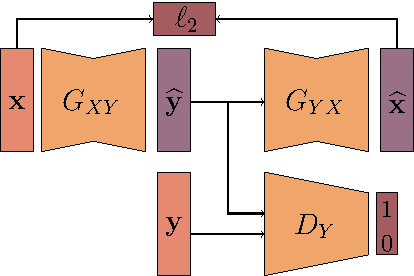
\includegraphics[width=\textwidth*3/5]{chapter1/cyclegan}
	\caption[CycleGAN approach]{The CycleGAN approach. Half of the training setup is illustrated, the other half consisting in the same setup but with inverted $\vx$ and $\vy$}
	\label{fig:cyclegan}
\end{figure}

A solution to this problem of paired data was proposed in the form of cyclic consistency \citep{Zhu2017, Kim2017,  Yi2018, Liu2018a}. Instead of training a single model $\G_{XY}$ with a reconstruction loss between $\vx$ and $\G(\vy)$, the cycle-consistent approaches train two domain-transfer models simultaneously: $\Gyx$ and $\Gxy$ that map samples from $\p{Y}$ onto $\p{X}$ and $\p{Y}$ onto $\p{X}$, respectively (\seefigure{fig:cyclegan}). This allows to compute the reconstruction errors  $||\vx - \Gyx(\Gxy(\vx))||_1$ and $||\vy - \Gxy(\Gyx(\vy))||_1$, which ensures that the semantic information is preserved through the mappings.  Note that these reconstruction errors never require paired data $(\vx,\vy)$. 

The training of the two models in done an adversarial setup, with two discriminators $\Dx$ and $\Dy$, and is summed up in the \textbf{\ac{CycleGAN}} approach \citep{Zhu2017},  formulated as

\begin{align}
	\label{eq:cyclegan}
	\min_{\Gxy, \Gyx}\max_{\Dx, \Dy} & \lcycgan  (\G_{XY}, \G_{YX}, \D_X, \D_Y) = \nonumber \\ 
	\min_{\Gxy, \Gyx}\max_{\Dx, \Dy}  &\esp{\vx\sim\p{\vx}}   \Big[(1-\D_X(\vx)^2) + (\D_Y(\G_{XY}(\vx)))^2 \Big] + \esp{y\sim\p{\vy}}  \Big[(1-\D_Y(\vy))^2 + (\D_X(\Gyx(\vy)))^2 \Big] \nonumber \\
	& +\lambda \Big[ \esp{\vx\sim\p{\vx}} ||\vx - \Gyx(\Gxy(\vx))||_1 + \esp{y\sim\p{\vy}} ||\vy - \Gxy(\Gyx(\vy))||_1 \Big] \enspace .
\end{align}

Note that instead of the classical \ac{GAN} losses, \ac{CycleGAN} uses the \ac{LSGAN} \citep{Mao2017} (see Section \ref{sec:divergences}) least-squares loss. The \ac{CycleGAN} training process then consists in alternatively updating the two discriminator and the two generators via gradient ascent/descent. A summary of this process is presented in \citealg{alg:cyclegan_train}. 

\ac{CycleGAN}, as well as similar methods relying on cycle-consistency such as \textbf{DualGAN} \citep{Yi2018} or \textbf{DiscoGAN} \citep{Kim2017}, have been used in a lot of domains such as medical imaging \citep{Chen2019}, training models with synthetic images (such as data obtained with a simulator, for example for robot grasping \citep{Bousmalis2018}), for image segmentation \citep{Perone2019}. More related to our domain, it has also been used by \citet{Sun2019} for converting near-infrared images to color images, which shows that conversion between different image modalities can be done with cycle-consistent generative models.


\begin{algorithm}[!t]
	\begin{algorithmic}[]
		\REQUIRE{$\trainsetX$ and $\trainsetY$ two unpaired datasets, $\Gxy$ and $\Gyx$ the mapping networks, $\Dx$ and $\Dy$ the discrimination models, $m$ the mini-batch size, $\lambda$ a hyperparameter}
		\REPEAT
		\STATE sample a mini-batch $\lbrace \vx_i \rbrace_{i=1}^m$ from $\trainsetX$\;
		\STATE sample a mini-batch $\lbrace \vy_i \rbrace_{i=1}^m$ from $\trainsetY$\;
		\STATE update $\Dx$ by stochastic gradient descent of
		\STATE \ \ \ \ $ \sum_{i=1}^{m}\big(\Dx(\vx_i)-1)^2 + \big(\Dx(\Gyx(\vy_i))\big)^2$
		\STATE update $\Dy$ by stochastic gradient descent of
		\STATE \ \ \ \ $ \sum_{i=1}^{m}\big(\Dy(\vy_i)-1)^2 + (\Dy(\Gxy(\vx_i)))^2$
		\STATE sample a mini-batch $\lbrace \vx_i \rbrace_{i=1}^m$ from $\trainsetX$\;
		\STATE sample a mini-batch $\lbrace \vy_i \rbrace_{i=1}^m$ from $\trainsetY$\;
		\STATE update $\Gxy$ by stochastic gradient descent of
		\STATE \ \ \ \ $ \sum_{i=1}^n \big(\Dy(\Gxy(\vx_i))-1\big)^2 + \lambda \big(||\vx_i - \Gyx(\Gxy(\vx_i))||_1 +||\vy_i -\Gxy(\Gyx(\vy_i))||_1\big)$\;
		\STATE update $\Gyx$ by stochastic gradient descent of
		\STATE \ \ \ \ $ \sum_{i=1}^n \big(\Dx(\Gyx(\vy_i))-1\big)^2+ \lambda\big (||\vx_i - \Gyx(\Gxy(\vx_i))||_1 + ||\vy_i - \Gxy(\Gyx(\vy_i))||_1\big)$\;
		\UNTIL a stopping condition is met
	\end{algorithmic}
	\caption{CycleGAN training algorithm}
	\label{alg:cyclegan_train}
\end{algorithm}




\section{Conclusion}



